\chapter{Wymagania}

\section{Diagram kontekstu}
\begin{figure}[h!]
    \centering
    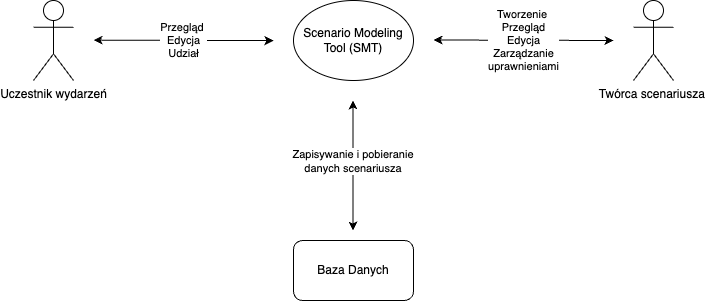
\includegraphics[width=0.99\textwidth]{resources/local/diagram-kontekstu.png}
    \caption{Diagram kontekstu}
\end{figure}

\section{Aktorzy}

\subsection{Twórca scenariusza}
Twórca scenariusza to osoba, która jest odpowiedzialna za tworzenie scenariuszy i ich modyfikowanie oraz dostosowywanie. 
Ma on możliwość definiowania wątków, obiektów, typów obiektów, szablonów, asocjacji, a także faz scenariusza w zależności 
od potrzeb i wymagań. Twórca scenariuszy może również nadawać uprawnienia edycji lub podglądu innym użytkownikom.

\subsection{Uczestnik wydarzeń}
Uczestnik wydarzeń to osoba biorąca udział w ćwiczeniach. Otrzymuje on dostęp do przeglądania lub modyfikacji scenariusza, 
w zależności od nadanych uprawnień. Dzięki temu podziałowi system jest odporny na wszelkie próby naruszenia integralności danych.

\section{Obiekty biznesowe}

\subsection{Scenariusz}
Scenariusz reprezentuje złożoną strukturę organizacyjną służącą do modelowania i symulacji sekwencji wydarzeń zachodzących 
w określonych ramach czasowych. Jest to centralny element systemu, który integruje i zarządza wieloma powiązanymi komponentami: 
wydarzeniami, wątkami, fazami i obiektami. Sam bezpośrednio zawiera metadane opisujące jego kontekst. 
Za jego pomocą zaimplementowany jest system uprawnień kontrolujący dostęp użytkowników.

\subsection{Faza scenariusza}
Faza scenariusza reprezentuje logiczny, wydzielony przedział czasowy w ramach całego scenariusza. 
Pozwala na podział scenariusza na mniejsze, znaczące etapy, ułatwiając organizację i wizualizację wydarzeń.

\subsection{Typ}

Typy służą do kategoryzacji i definiowania zasad zachowania elementów w systemie. Stanowią podstawę do zachowania spójności 
i prawidłowych relacji między elementami w systemie. Wyróżniamy dwa podstawowe rodzaje:
\begin{itemize}
    \item Typ Obiektu - jest to definicja kategorii obiektu występującego w scenariuszu. 
    Określa jego podstawowe cechy i zachowania, w tym konieczność globalnego dostępu do obiektu, 
    możliwość przypisania do niego użytkownika czy przynależność do szerszej kategorii (występuje hierarchia).
    \item Typ Asocjacji - Definiuje dozwolony rodzaj relacji między obiektami w systemie. 
    Określa typy obiektów które mogą wchodzić ze sobą w interakcje.
\end{itemize}

\subsection{Szablon}

Szablony definiują wzorce dla obiektów i ich atrybutów, umożliwiając standaryzację i automatyzację procesu tworzenia nowych 
elementów w scenariuszach.

\begin{itemize}
    \item Szablon Obiektu - Stanowi wzorzec definiujący strukturę i domyślne właściwości dla grupy podobnych obiektów. 
    Określa zarówno typ obiektu, do którego jest przypisany jak i wymagane atrybuty.
    \item Szablon Atrybutu - Definiuje pojedynczą cechę, którą mogą posiadać obiekty danego szablonu.
    Szablony pozwalają na szybkie i spójne tworzenie nowych elementów w systemie, zapewniając standardowy zestaw właściwości 
    i wartości początkowych.
\end{itemize}

\subsection{Obiekt}

Obiekt stanowi podstawową jednostkę w scenariuszu, reprezentującą konkretny element posiadający zdefiniowane atrybuty i 
mogący wchodzić w relacje z innymi obiektami. System rozróżnia obiekty globalne tworzone w wątku globalnym i dostępne w każdym 
innym oraz obiekty lokalne przypisane do konkretnych wątków i niedostępne w danym czasie w żadnym innym. 
Jedynym sposobem ich przekazania dalej są operacje rozgałęzień na wątkach.
Każdy obiekt tworzony jest na podstawie szablonu określającego jego strukturę.

\subsection{Asocjacja}

Asocjacje reprezentują relacje między obiektami w scenariuszu. Mogą być tworzone i usuwane w ramach wydarzeń.

\subsection{Atrybut}

Atrybuty definiują właściwości obiektów, które mogą zmieniać się w czasie trwania scenariusza. Każdy atrybut jest tworzony 
na podstawie szablonu obiektu określającego jego cechy domyślnie przyjmuje wartość zdefiniowaną w szablonie.

\subsection{Wątek}

Wątek reprezentuje sekwencję wydarzeń w scenariuszu, pozwalając na modelowanie równoległych ciągów wydarzeń. 
Trwają określoną liczbę akcji. W systemie występują dwa rodzaje wątków:
\begin{itemize}
    \item Wątek Globalny:
    \begin{itemize}
        \item Jest jeden na scenariusz,
        \item Zawiera wydarzenia globalne wpływające na wszystkie pozostałe wątki,
        \item Przechowuje obiekty globalne dostępne w całym scenariuszu.
    \end{itemize}
    \item Wątki Lokalne:
    \begin{itemize}
        \item Reprezentują niezależne sekwencje wydarzeń,
        \item Zawierają własne, lokalne obiekty,
        \item Mogą być łączone lub rozdzielane za pomocą rozgałęzień.
    \end{itemize}
\end{itemize}

\subsection{Rozgałęzienie}

Wątki mogą na siebie oddziaływać poprzez operacje:
\begin{itemize}
    \item FORK - podział jednego wątku na wiele, wraz z dystrybucją obiektów - definiowaną przez użytkownika.
    \item JOIN - łączenie wielu wątków w jeden, wraz z przekazaniem ich obiektów.
\end{itemize}

\subsection{Wydarzenie}

Wydarzenie trwa zawsze jedną akcję. Opisuje zachodzące w określonym momencie scenariusza zmiany (także te wpływające na organizację 
wątków). System rozróżnia następujące typy wydarzeń:
\begin{itemize}
    \item START/END - kontrolują rozpoczęcie i zakończenie wątku.
    \item NORMAL - standardowe wydarzenia w wątku lokalnym.
    \item GLOBAL - wydarzenia w wątku globalnym (najwyższy priorytet).
    \item FORK\_IN/FORK\_OUT - obsługują proces podziału wątku.
    \item JOIN\_IN/JOIN\_OUT - obsługują proces łączenia wątków.
    \item IDLE - wydarzenia puste, brak zmian w wątku.
\end{itemize}

Tylko wydarzenia IDLE, NORMAL oraz GLOBAL są bezpośrednio tworzone przez użytkownika. 
W wydarzeniach NORMAL oraz GLOBAL następują modyfikacje atrybutów obiektów oraz zarządzanie asocjacjami między nimi.

\newpage
\section{Diagram przypadków użycia}
\begin{figure}[h!]
    \centering
    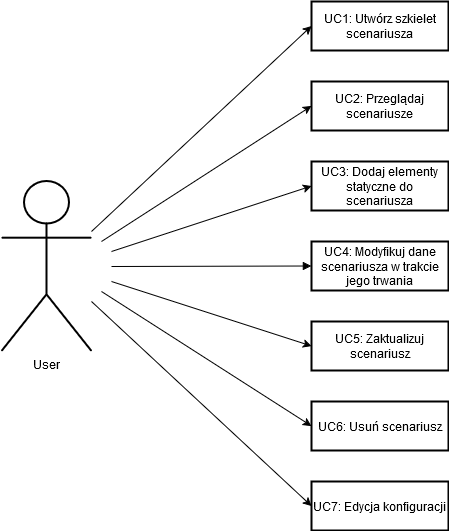
\includegraphics[width=0.5\textwidth]{resources/local/use-case-diagram-2.png}
    \caption{Diagram przypadków użycia}
    \label{fig:use_case_diagram}
\end{figure}

\section{Tabela przypadków użycia}
\small{
\begin{longtable}{|p{1cm}|p{4.5cm}|p{8cm}|}
    \hline
    \textbf{ID} & \textbf{Przypadek użycia} & \textbf{Opis} \\
    \hline
    \endfirsthead
    \caption[]{Tabela przypadków użycia -- ciąg dalszy} \\
    \hline
    \textbf{ID} & \textbf{Przypadek użycia} & \textbf{Opis} \\
    \hline
    \endhead
    \hline
    \endfoot
    \hline
    \caption{Tabela przypadków użycia} \label{tab:use_case_table} \\
    \endlastfoot
    UC1 & Utwórz szkielet scenariusza & Użytkownik tworzy scenariusz podając jego czas wraz z pozostałymi właściwościami go opisującymi. System dodaje nowy scenariusz wraz z domyślnymi danymi tworzonymi dla nowego scenariusza. \\
    \hline
    UC2 & Przeglądaj scenariusze & Użytkownik przegląda listę dostępnych scenariuszy, z opcją filtrowania, która umożliwia wybranie konkretnego scenariusza oraz jego edycję lub usunięcie. \\
    \hline
    UC3.1 & Utwórz szablon obiektu & Użytkownik tworzy szablon obiektu dostępny we wszystkich scenariuszach. \\
    \hline
    UC3.2 & Utwórz obiekt & Użytkownik tworzy konkretny obiekt przypisany do scenariusza. \\
    \hline
    UC3.3 & Utwórz szablon atrybutu & Użytkownik tworzy szablon atrybutu przyporządkowany do danego szablonu obiektu. \\
    \hline
    UC3.4 & Utwórz typ obiektu & Użytkownik tworzy typ obiektu dostępny we wszystkich scenariuszach. \\
    \hline
    UC3.5 & Utwórz typ asocjacji & Użytkownik tworzy typ asocjacji dostępny we wszystkich scenariuszach. \\
    \hline
    UC3.6 & Utwórz asocjację & Użytkownik tworzy asocjację pomiędzy dwoma obiektami z danego scenariusza. \\
    \hline
    UC4.1 & Utwórz wątek & Użytkownik tworzy nowy wątek poprzez rozdzielenie wątku istniejącego lub dodanie nowego osobnego wątku. \\
    \hline
    UC4.2 & Utwórz zdarzenie & Użytkownik tworzy zdarzenie wraz ze zdefiniowaniem zmian w asocjacjach lub atrybutach obiektów. \\
    \hline
    UC5.1 & Edycja danych podanych przy tworzeniu scenariusza & Użytkownik modyfikuje właściwości scenariusza podane podczas jego tworzenia. \\
    \hline
    UC5.2 & Edycja elementów statycznych oraz zdarzeń & Użytkownik modyfikuje istniejące elementy statyczne (np. obiekty, atrybuty) wraz z właściwościami zdarzeń i wątków. \\
    \hline
    UC.6.1 & Usuń scenariusz & Użytkownik usuwa scenariusz po jego wybraniu z listy. System pyta o potwierdzenie i usuwa scenariusz wraz z danymi prywatnymi dla scenariusza na stałe. \\
    \hline
    UC.6.2 & Usuń element statyczny & Użytkownik posiada opcję usunięcia: typu asocjacji oraz obiektu, szablonu obiektu oraz atrybutu, konkretnego obiektu, wątku, rozgałęzienia i fazy.    \\
    \hline
    UC.7 & Edycja konfiguracji & Użytkownik edytuje konfigurację. System wykorzystuje zdefiniowane właściwości przy tworzeniu nowego scenariusza. \\
    \hline
\end{longtable}
}
\normalsize
\section{Wymagania pozafunkcjonalne}
Wymagania pozafunkcjonalne są zgodne ze standardem ISO 25010, zdefiniowanym w książce 
\emph{Systems and Software Engineering — Systems and Software Quality Requirements and Evaluation (SQuaRE) — System and Software Quality Models} 
\cite{iso25010} i zostały opisane w poniższej tabeli:

\section{Tabela wymagań pozafunkcjonalnych}
\small{
\begin{longtable}{|p{1cm}|p{2.5cm}|p{4.5cm}|p{5cm}|}
    \hline
    \textbf{ID} & \textbf{ISO 25010} & \textbf{Wymaganie} & \textbf{Realizacja} \\
    \hline
    \endfirsthead
    \caption[]{Tabela wymagań pozafunkcjonalnych -- ciąg dalszy} \\
    \hline
    \textbf{ID} & \textbf{ISO 25010} & \textbf{Wymaganie} & \textbf{Realizacja} \\
    \hline
    \endhead
    \hline
    \endfoot
    \hline
    \caption{Tabela wymagań pozafunkcjonalnych} \label{tab:NFR-table} \\
    \endlastfoot
    NFR1 & Funkcjonalność & System powinien dostarczać wszystkie wymagane funkcje. & Implementacja zgodnie z przedstawionymi wymaganiami.\\
    \hline
    NFR2 & Funkcjonalność & Funkcje systemowe powinny działać zgodnie z wymaganiami dostarczając odpowiednie odpowiedzi. & Sprawdzenie przy pomocy testów integracyjnych i jednostkowych. \\
    \hline
    NFR3 & Wydajność & Aplikacja powinna umożliwiać efektywne zarządzanie żądaniami. &  Osiągnięte dzięki optymalizacji transakcji i dostępu do bazy danych poprzez wykorzystanie mechanizmu keylock w celu unikania konfliktów podczas równoczesnego dostępu do danych. \\
    \hline
    NFR4 & Wydajność & System musi spełniać wymóg skalowalności w celu obsługi wielu użytkowników bez znaczącego spadku wydajności. & Realizacja poprzez zastosowanie mikroserwisową architekturę. \\
    \hline
    NFR5 & Zgodność & System powinien współpracować z innymi systemami. & Osiągnięte dzięki wykorzystaniu websocketa oraz integracji za pomocą REST API. \\
    \hline
    NFR6 & Zgodność & System powinien działać na różnych urządzeniach. & Zapewnienie responsywności poprzez implementację za pomocą CSS Media Queries. \\
    \hline
    NFR7 & Użyteczność & Aplikacja powinna zapewniać rozpoznawalność zastosowania. & Umożliwiło to zastosowanie czytelnego układu oraz zgodności z UX. \\
    \hline
    NFR8 & Użyteczność & System powinien zawierać czytelny i intuicyjny interfejs. & Realizacja przy użyciu frameworka React oraz komponentów w standardzie WCAG 2.1. \\
    \hline
    NFR9 & Użyteczność & System powinien odpowiednio stosować semantykę HTML. & Wykorzystanie odpowiednich znaczników HTML oraz frameworków, które wspierają A11y. \\
    \hline
    NFR10 & Użyteczność & Użytkownik powinien mieć pełną kontrolę za pomocą klawiatury. & Przeprowadzenie testów wszystkich komponentów aplikacji przy pomocy klawiatury. \\
    \hline
    NFR11 & Niezawodność & Aplikacja powinna radzić sobie z błędami. & Aplikacja zawiera system obsługi wyjątków oraz testy end to end. \\
    \hline
    NFR12 & Niezawodność & Kod aplikacji powinien zapewniać transakcyjność oraz integralność danych. & Wykorzystanie PostgreSQL, który umożliwia kontrolę integralności oraz operacja transakcyjne. \\
    \hline
    NFR13 & Łatwość utrzymania & System powinien spełniać zasady SOLID oraz modularność. & Uzyskanie poprzez implementację według zasad SOLID, co umożliwia łatwe dodawanie nowych funkcji. \\
    \hline
    NFR14 & Łatwość utrzymania & Zmiany logiki w warstwie nie powinny wymagać zmian w pozostałych warstwach. &  Zastosowanie odpowiedniej architektury wartstowej. \\
    \hline
    NFR15 & Łatwość utrzymania & System powinien być przystosowany do automatycznego testowania. & Wykorzystanie testów jednostkowych oraz testów end-to-end. \\
    \hline
    NFR16 & Bezpieczeństwo & Aplikacja powinna zawierać odpowiednie mechanizmy uwierzytelniania i autoryzacji. & Implementacja mechnizmów JWT oraz uprawienia użytkowników na podstawie ich ról. \\
    \hline
    NFR17 & Bezpieczeństwo & System powinien zwracać logi. & Dodanie kodów błędów na poziomie API Exception. \\
    \hline
    NFR18 & Przenośność  & System powinien być łatwy do wdrożenia w różnych środowiskach. & Wykorzystanie Dockera i Docker Compose.\\
    \hline
    NFR19 & Przenośność & Aplikacja powinna łatwa do uruchomienia. & Zastosowanie konteneryzacji oraz gotwych skryptów. \\
    \hline
\end{longtable}
}
\normalsize